\documentclass[]{article}
\usepackage{lmodern}
\usepackage{amssymb,amsmath}
\usepackage{ifxetex,ifluatex}
\usepackage{fixltx2e} % provides \textsubscript
\ifnum 0\ifxetex 1\fi\ifluatex 1\fi=0 % if pdftex
  \usepackage[T1]{fontenc}
  \usepackage[utf8]{inputenc}
\else % if luatex or xelatex
  \ifxetex
    \usepackage{mathspec}
  \else
    \usepackage{fontspec}
  \fi
  \defaultfontfeatures{Ligatures=TeX,Scale=MatchLowercase}
\fi
% use upquote if available, for straight quotes in verbatim environments
\IfFileExists{upquote.sty}{\usepackage{upquote}}{}
% use microtype if available
\IfFileExists{microtype.sty}{%
\usepackage{microtype}
\UseMicrotypeSet[protrusion]{basicmath} % disable protrusion for tt fonts
}{}
\usepackage[margin=1in]{geometry}
\usepackage{hyperref}
\hypersetup{unicode=true,
            pdftitle={create a TS diagram as a ggplot},
            pdfauthor={David Kaiser},
            pdfborder={0 0 0},
            breaklinks=true}
\urlstyle{same}  % don't use monospace font for urls
\usepackage{color}
\usepackage{fancyvrb}
\newcommand{\VerbBar}{|}
\newcommand{\VERB}{\Verb[commandchars=\\\{\}]}
\DefineVerbatimEnvironment{Highlighting}{Verbatim}{commandchars=\\\{\}}
% Add ',fontsize=\small' for more characters per line
\usepackage{framed}
\definecolor{shadecolor}{RGB}{248,248,248}
\newenvironment{Shaded}{\begin{snugshade}}{\end{snugshade}}
\newcommand{\KeywordTok}[1]{\textcolor[rgb]{0.13,0.29,0.53}{\textbf{#1}}}
\newcommand{\DataTypeTok}[1]{\textcolor[rgb]{0.13,0.29,0.53}{#1}}
\newcommand{\DecValTok}[1]{\textcolor[rgb]{0.00,0.00,0.81}{#1}}
\newcommand{\BaseNTok}[1]{\textcolor[rgb]{0.00,0.00,0.81}{#1}}
\newcommand{\FloatTok}[1]{\textcolor[rgb]{0.00,0.00,0.81}{#1}}
\newcommand{\ConstantTok}[1]{\textcolor[rgb]{0.00,0.00,0.00}{#1}}
\newcommand{\CharTok}[1]{\textcolor[rgb]{0.31,0.60,0.02}{#1}}
\newcommand{\SpecialCharTok}[1]{\textcolor[rgb]{0.00,0.00,0.00}{#1}}
\newcommand{\StringTok}[1]{\textcolor[rgb]{0.31,0.60,0.02}{#1}}
\newcommand{\VerbatimStringTok}[1]{\textcolor[rgb]{0.31,0.60,0.02}{#1}}
\newcommand{\SpecialStringTok}[1]{\textcolor[rgb]{0.31,0.60,0.02}{#1}}
\newcommand{\ImportTok}[1]{#1}
\newcommand{\CommentTok}[1]{\textcolor[rgb]{0.56,0.35,0.01}{\textit{#1}}}
\newcommand{\DocumentationTok}[1]{\textcolor[rgb]{0.56,0.35,0.01}{\textbf{\textit{#1}}}}
\newcommand{\AnnotationTok}[1]{\textcolor[rgb]{0.56,0.35,0.01}{\textbf{\textit{#1}}}}
\newcommand{\CommentVarTok}[1]{\textcolor[rgb]{0.56,0.35,0.01}{\textbf{\textit{#1}}}}
\newcommand{\OtherTok}[1]{\textcolor[rgb]{0.56,0.35,0.01}{#1}}
\newcommand{\FunctionTok}[1]{\textcolor[rgb]{0.00,0.00,0.00}{#1}}
\newcommand{\VariableTok}[1]{\textcolor[rgb]{0.00,0.00,0.00}{#1}}
\newcommand{\ControlFlowTok}[1]{\textcolor[rgb]{0.13,0.29,0.53}{\textbf{#1}}}
\newcommand{\OperatorTok}[1]{\textcolor[rgb]{0.81,0.36,0.00}{\textbf{#1}}}
\newcommand{\BuiltInTok}[1]{#1}
\newcommand{\ExtensionTok}[1]{#1}
\newcommand{\PreprocessorTok}[1]{\textcolor[rgb]{0.56,0.35,0.01}{\textit{#1}}}
\newcommand{\AttributeTok}[1]{\textcolor[rgb]{0.77,0.63,0.00}{#1}}
\newcommand{\RegionMarkerTok}[1]{#1}
\newcommand{\InformationTok}[1]{\textcolor[rgb]{0.56,0.35,0.01}{\textbf{\textit{#1}}}}
\newcommand{\WarningTok}[1]{\textcolor[rgb]{0.56,0.35,0.01}{\textbf{\textit{#1}}}}
\newcommand{\AlertTok}[1]{\textcolor[rgb]{0.94,0.16,0.16}{#1}}
\newcommand{\ErrorTok}[1]{\textcolor[rgb]{0.64,0.00,0.00}{\textbf{#1}}}
\newcommand{\NormalTok}[1]{#1}
\usepackage{graphicx,grffile}
\makeatletter
\def\maxwidth{\ifdim\Gin@nat@width>\linewidth\linewidth\else\Gin@nat@width\fi}
\def\maxheight{\ifdim\Gin@nat@height>\textheight\textheight\else\Gin@nat@height\fi}
\makeatother
% Scale images if necessary, so that they will not overflow the page
% margins by default, and it is still possible to overwrite the defaults
% using explicit options in \includegraphics[width, height, ...]{}
\setkeys{Gin}{width=\maxwidth,height=\maxheight,keepaspectratio}
\IfFileExists{parskip.sty}{%
\usepackage{parskip}
}{% else
\setlength{\parindent}{0pt}
\setlength{\parskip}{6pt plus 2pt minus 1pt}
}
\setlength{\emergencystretch}{3em}  % prevent overfull lines
\providecommand{\tightlist}{%
  \setlength{\itemsep}{0pt}\setlength{\parskip}{0pt}}
\setcounter{secnumdepth}{0}
% Redefines (sub)paragraphs to behave more like sections
\ifx\paragraph\undefined\else
\let\oldparagraph\paragraph
\renewcommand{\paragraph}[1]{\oldparagraph{#1}\mbox{}}
\fi
\ifx\subparagraph\undefined\else
\let\oldsubparagraph\subparagraph
\renewcommand{\subparagraph}[1]{\oldsubparagraph{#1}\mbox{}}
\fi

%%% Use protect on footnotes to avoid problems with footnotes in titles
\let\rmarkdownfootnote\footnote%
\def\footnote{\protect\rmarkdownfootnote}

%%% Change title format to be more compact
\usepackage{titling}

% Create subtitle command for use in maketitle
\newcommand{\subtitle}[1]{
  \posttitle{
    \begin{center}\large#1\end{center}
    }
}

\setlength{\droptitle}{-2em}
  \title{create a TS diagram as a ggplot}
  \pretitle{\vspace{\droptitle}\centering\huge}
  \posttitle{\par}
  \author{David Kaiser}
  \preauthor{\centering\large\emph}
  \postauthor{\par}
  \predate{\centering\large\emph}
  \postdate{\par}
  \date{2018/01/16}


\begin{document}
\maketitle

\subsubsection{Description}\label{description}

A TS diagram, Temperature-Salinity-diagram, plots the \textbf{potential
temperature} of water over \textbf{salinity}. Many water masses have
characteristic shapes in a TS diagram, which is used in physical
oceanography to identify water masses and their mixing (see e.g.
\url{https://doi.org/10.1016/S0422-9894(08)71172-3}).

This function requires the input of vectors of \textbf{potential
temperature} and \textbf{salinity}. The \emph{gws} package is used to
calculate potential density for plotting of isopycnals (contours of the
same density). This calculation requires a \textbf{reference pressure},
which defaults to 0, the sea surface.

A third vector can optionally be supplied to \textbf{col.par} to be
plotted in color, and can be named with a string supplied to
\textbf{col.name}.

\subsubsection{Arguments}\label{arguments}

\emph{sal} -- vector of salinity values

\emph{pot.temp} -- vector of potential temperature values in degree C

\emph{reference.p = 0} -- reference pressure which was also used to
calculate potential temperature

\emph{col.par = NA} -- optional vector of a parameter to be displayed as
color of the TS-pairs

\emph{col.name = ``col.par''} -- optional name of the ``col.par'' to be
used on the color bar

\subsubsection{Plot}\label{plot}

\begin{Shaded}
\begin{Highlighting}[]
\NormalTok{example <-}\StringTok{ }\KeywordTok{read.csv}\NormalTok{(}\StringTok{"example_data/example_data.csv"}\NormalTok{)}

\KeywordTok{head}\NormalTok{(example)}
\end{Highlighting}
\end{Shaded}

\begin{verbatim}
##   X depth potential.temperature salinity
## 1 1  1.50                6.1272  13.2087
## 2 2  1.75                6.1245  13.2115
## 3 3  2.00                6.1236  13.2128
## 4 4  2.25                6.1227  13.2126
## 5 5  2.50                6.1229  13.2145
## 6 6  2.75                6.1224  13.2122
\end{verbatim}

The data will be plotted using the \emph{ggplot2} package.

\begin{Shaded}
\begin{Highlighting}[]
\KeywordTok{ggTS_DK}\NormalTok{(}\DataTypeTok{sal =}\NormalTok{ example}\OperatorTok{$}\NormalTok{salinity, }
        \DataTypeTok{pot.temp =}\NormalTok{ example}\OperatorTok{$}\NormalTok{potential.temperature, }
        \DataTypeTok{reference.p =} \DecValTok{0}\NormalTok{,}
        \DataTypeTok{col.par =}\NormalTok{ example}\OperatorTok{$}\NormalTok{depth, }
        \DataTypeTok{col.name =} \StringTok{"depth [m]"}\NormalTok{)}
\end{Highlighting}
\end{Shaded}

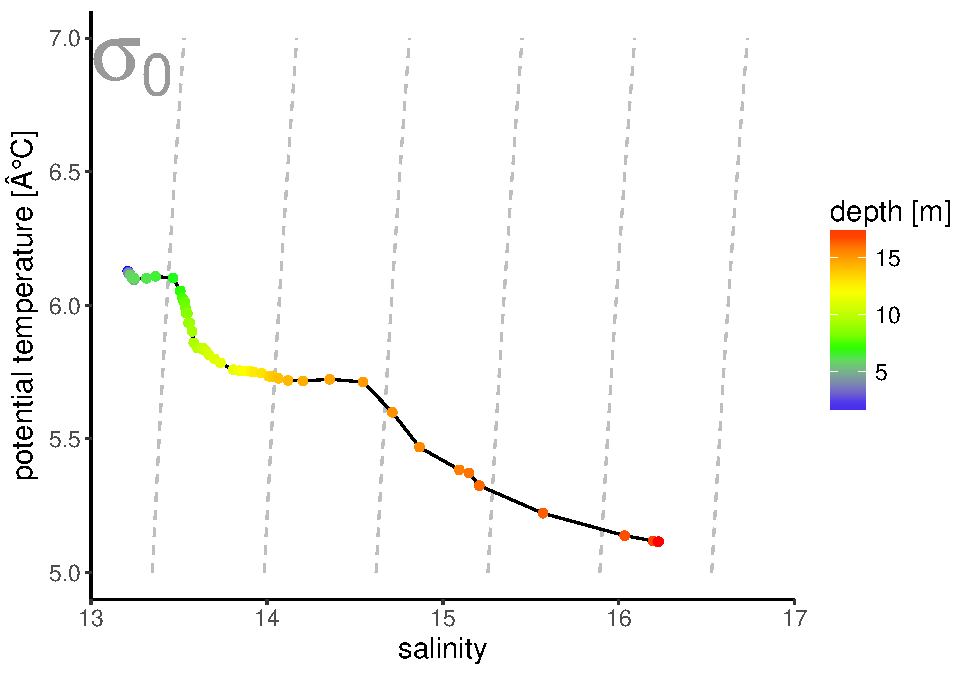
\includegraphics{README_files/figure-latex/plot_result-1.pdf}

\textbf{NOTE}: the special ``Â'' character does not show when the
function is used in R, this seems to be a markdown/knitr problem

Since the result is a ggplot, it can be altered and amended:

\begin{Shaded}
\begin{Highlighting}[]
\NormalTok{p1 <-}\StringTok{ }\KeywordTok{ggTS_DK}\NormalTok{(}\DataTypeTok{sal =}\NormalTok{ example}\OperatorTok{$}\NormalTok{salinity, }
        \DataTypeTok{pot.temp =}\NormalTok{ example}\OperatorTok{$}\NormalTok{potential.temperature, }
        \DataTypeTok{reference.p =} \DecValTok{0}\NormalTok{,}
        \DataTypeTok{col.par =}\NormalTok{ example}\OperatorTok{$}\NormalTok{depth, }
        \DataTypeTok{col.name =} \StringTok{"depth [m]"}\NormalTok{)}
\NormalTok{p1 }\OperatorTok{+}\StringTok{ }\KeywordTok{scale_color_gradient}\NormalTok{(}\DataTypeTok{low =} \StringTok{"grey"}\NormalTok{, }\DataTypeTok{high =} \StringTok{"black"}\NormalTok{, }\DataTypeTok{name =} \StringTok{"something}\CharTok{\textbackslash{}n}\StringTok{else"}\NormalTok{) }\OperatorTok{+}
\StringTok{      }\KeywordTok{annotate}\NormalTok{(}\DataTypeTok{geom =} \StringTok{"text"}\NormalTok{, }\DataTypeTok{x =} \DecValTok{15}\NormalTok{, }\DataTypeTok{y =} \DecValTok{6}\NormalTok{, }\DataTypeTok{color =} \StringTok{"red"}\NormalTok{, }\DataTypeTok{size =} \DecValTok{14}\NormalTok{, }\DataTypeTok{label =} \StringTok{"ADD}\CharTok{\textbackslash{}n}\StringTok{STUFF"}\NormalTok{)}
\end{Highlighting}
\end{Shaded}

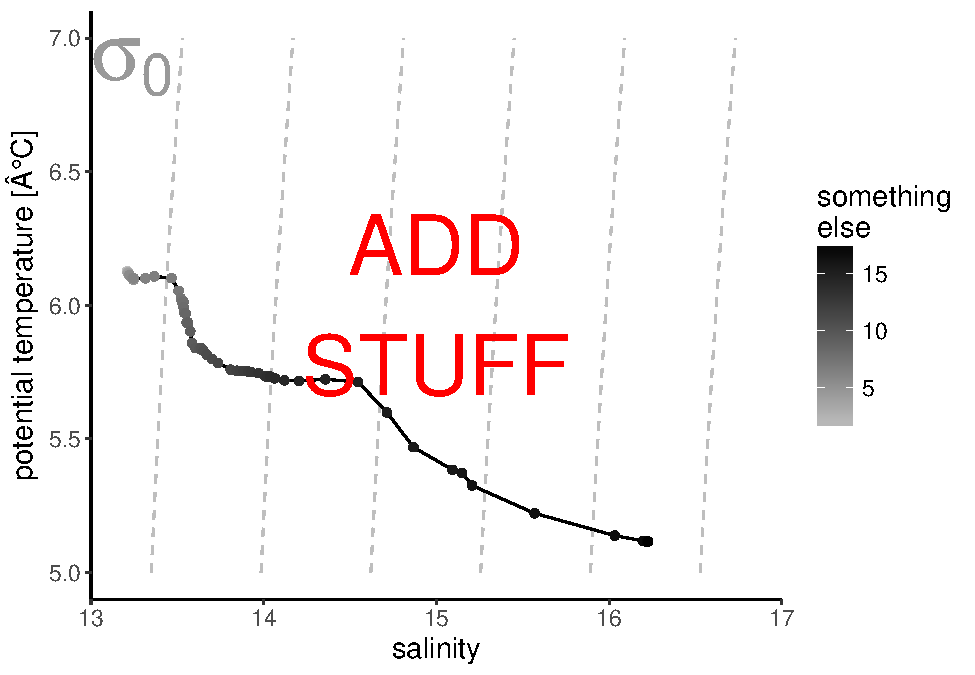
\includegraphics{README_files/figure-latex/extenden_plot-1.pdf}

\subsubsection{in preparation}\label{in-preparation}

\textbf{Isopycnal labels}: Currently the isopycnals are not labeled in
the example. For cases in which the isopycnals run fairly horizontally
through the plot and cut through its right side edge, and in which the
calculated potential density range is large enough, this works already.
But this is not the case for the example data.


\end{document}
